\chapter{Channel Equalization: CTLE, FFE, DFE, and DSP}
\label{ch:equalization}
\label{sec:equalization}

This chapter is the design judgment home for short-reach equalization: what the
channel does to symbols, which impairments linear filters can fix, when
decision feedback helps, and how transmit versus receive FFE differ. Module
placement (retimed, LPO, redriver) and SerDes versus DSP vocabulary stay in
\Cref{sec:serdes-dsp,sec:conditioning}. Multilevel alphabet pressure is in
\Cref{ch:multilevel}. Noise and BER math are in \Cref{ch:models}.

\textit{Read first:} precursor versus postcursor, FFE versus DFE, TX versus RX
FFE, and the adaptation traps.

\textit{Deep dive:} TDECQ reference FFE in \Cref{sec:tdecq}; COM eye budgets in
\Cref{sec:eye-budget}.

\keyidea{FFE can clean up pre- and post-cursor ISI, but it may boost noise. DFE
avoids that noise boost for canceled post-cursors, but it can propagate bad
decisions. The first question is which impairment you are correcting, not which
acronym is fashionable.}

\section{Start from the channel}
\label{sec:eq-channel}

A short-reach lane is a lossy, reflective, discontinuous filter. Before you name
an equalizer, name the impairment:

\begin{description}
\item[Frequency-dependent loss] Skin effect and dielectric loss tilt the
      spectrum. High-frequency edges arrive weaker than low-frequency content.
\item[ISI] Energy from one symbol spills into neighbors. \emph{Precursor} ISI
      arrives before the main cursor; \emph{postcursor} ISI arrives after.
\item[Reflections] Package, connector, and cable discontinuities create echoes
      that look like delayed ISI.
\item[Crosstalk] Neighboring lanes add interference that equalization cannot
      fully undo if it is not in the equalizer's observation set.
\item[Noise enhancement] Linear boost that restores edges also amplifies
      high-frequency noise.
\item[Nonlinear distortion] Compression, duty-cycle distortion, and optical
      nonlinearities create errors that a linear equalizer cannot invert safely.
\end{description}

The central question:

\begin{quote}
\noindent Which impairments can be corrected linearly, which require decisions,
and which cannot be equalized safely?
\end{quote}

If the answer is ``the eye is closed by compression or by unobservable
crosstalk,'' adding taps is not a design win.

\subsection{Read the impulse response, not the acronym}
\label{sec:eq-impulse}

On a whiteboard, draw a discrete pulse response with a main cursor and a few
neighbors. Label:

\begin{itemize}
\item the cursor (the sample you want to keep),
\item precursors (samples before the cursor: future symbols leaking backward),
\item postcursors (samples after the cursor: past symbols still ringing).
\end{itemize}

That sketch decides the toolbox. Precursor energy forces FFE or TX
pre-emphasis. Postcursor energy can be attacked by FFE, DFE, or both. A smooth
one-pole tilt suggests CTLE first. A long ringing tail with reflections suggests
more taps and a hard look at package/connector discontinuities. If the ``ISI''
changes with optical bias or OMA, you are no longer in a pure electrical linear
channel (\Cref{sec:eq-optical}).

\begin{figure}[ht]
\centering
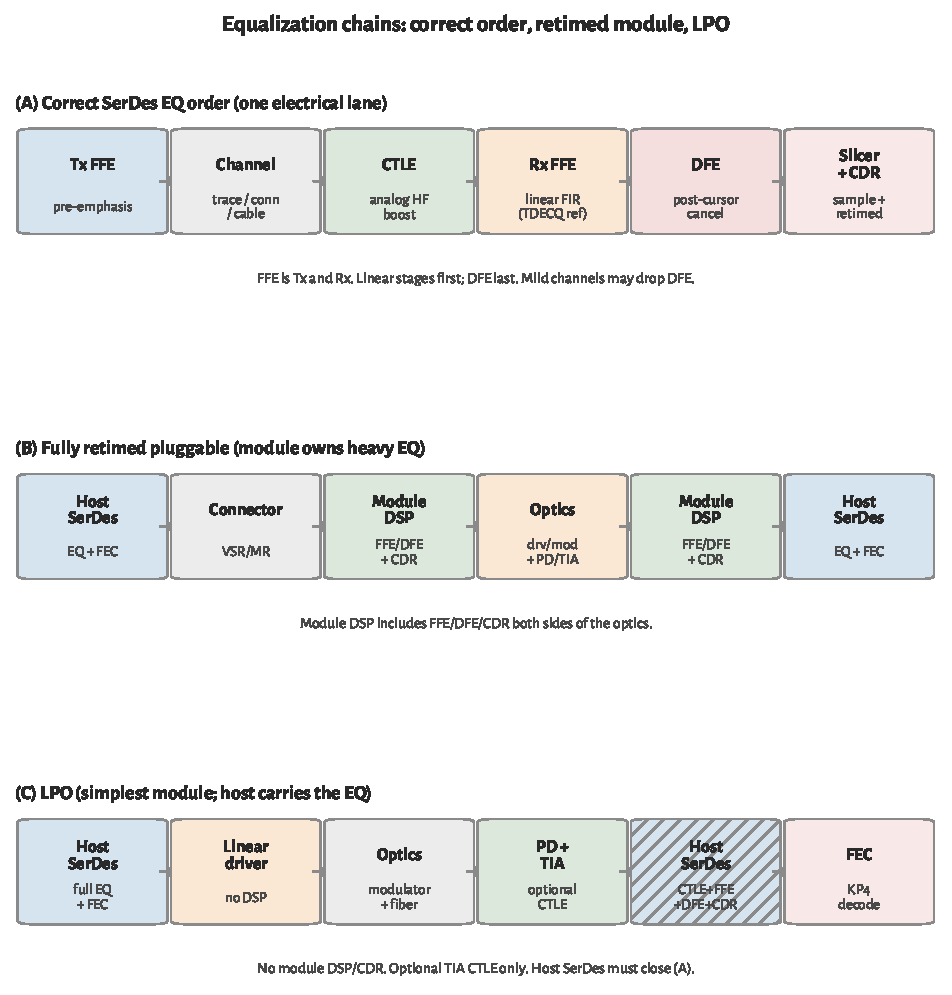
\includegraphics[width=\linewidth]{figures/fig_eq_chains.pdf}
\caption{Equalization chains. (A)~Correct order on one electrical lane: Tx FFE,
channel, CTLE, Rx FFE, DFE, then slicer/CDR. (B)~Fully retimed pluggable: module
DSP owns FFE/DFE/CDR on both sides of the optics. (C)~LPO: no module DSP; the host
SerDes must close the full EQ and FEC path.\label{fig:eq-chains}}
\end{figure}

\section{CTLE}
\label{sec:eq-ctle}

A \term{CTLE}\firstterm{CTLE} (continuous-time linear equalizer) boosts high
frequencies relative to low frequencies in the analog front end. It compensates
smooth channel loss with low complexity and low latency. It is friendly to
TIAs, redrivers, and SerDes peaking stages.

Limits:

\begin{itemize}
\item It also boosts high-frequency noise.
\item A fixed or coarsely tuned CTLE cannot match an arbitrary multipath
      response tap-by-tap.
\item Over-boost creates ringing that looks like new ISI.
\end{itemize}

Use CTLE as the first, cheap tilt correction. Do not ask it to replace a
full FFE/DFE story on a hostile channel.

In short-reach optics, CTLE often appears in three places: the host SerDes
front-end, a redriver or ACC mid-channel, and the module TIA peaking stage for
LPO. Those are not three independent free boosts. Stacking aggressive CTLE
stages can create peaking that looks open on a scope and still fails BER because
noise and ringing grew with the edge rate (\Cref{sec:conditioning,sec:serdes-dsp}).

\section{Feed-forward equalizer}
\label{sec:eq-ffe}

An \term{FFE}\firstterm{FFE} is a weighted sum of the current sample and its
neighbors:
\begin{equation}
y[n] = \sum_k c_k\, x[n-k].
\label{eq:ffe}
\end{equation}

It can correct precursor ISI, postcursor ISI, and a known linear channel
response when enough taps and resolution exist. Host SerDes and module DSPs use
FFE, often after CTLE. Transmitter quality metrics such as TDECQ apply a
\emph{bounded} reference FFE when scoring a waveform (\Cref{sec:tdecq}).

Think of the taps by role:

\begin{description}
\item[Main cursor] Sets the scale of the decision sample.
\item[Precursor taps] Cancel energy from future symbols. Required when the
      channel has advance ISI that DFE cannot see.
\item[Postcursor taps] Cancel lingering energy from past symbols without using
      decisions. They compete with DFE for the same impairment.
\end{description}

Costs:

\begin{itemize}
\item Linear filtering can amplify noise, especially with large high-frequency
      taps.
\item Many taps cost power, area, and latency.
\item Tap range and resolution matter: pegged taps mean the equalizer is out of
      authority.
\item Finite bit width on coefficients creates quantization that matters more as
      eyes shrink (PAM8 pressure in \Cref{ch:multilevel}).
\end{itemize}

A practical interview answer is not ``use more taps.'' It is ``use enough taps
to cover the significant pulse-response length, then stop when residual ISI is
smaller than the noise and nonlinearity you cannot equalize.''

\section{Decision-feedback equalizer}
\label{sec:eq-dfe}

A \term{DFE}\firstterm{DFE} uses past symbol decisions to subtract expected
postcursor ISI:
\begin{equation}
y[n] = x[n] - \sum_{k=1}^{N} b_k\,\hat{a}[n-k].
\label{eq:dfe}
\end{equation}

Advantages:

\begin{itemize}
\item It does not amplify front-end noise the same way an FFE does for the
      canceled postcursors.
\item It is effective when postcursor ISI dominates.
\end{itemize}

Limits:

\begin{itemize}
\item It cannot correct precursor ISI (those samples arrive before the
      decision).
\item Wrong decisions feed the filter: \emph{error propagation}.
\item The feedback loop must close quickly; timing and decision latency matter.
\item At very high baud rates, closing a long DFE loop is hard.
\end{itemize}

CEI electrical eye budgets often assume a reference DFE at the slicer
(\Cref{sec:eye-budget}). That is a compliance model, not proof that your product
DFE is healthy.

Error propagation is the main interview trap. One wrong decision subtracts the
wrong amount on later samples, which can create a short burst of additional
errors. That burst may still be correctable by FEC, or it may cluster into a
FEC-unfriendly pattern. When someone says ``DFE is free SNR,'' ask how the link
behaves when decisions are marginal, not only when the eye is wide open.

\section{FFE versus DFE}
\label{sec:eq-ffe-vs-dfe}

\begin{center}
\footnotesize
\begin{tabular}{@{}p{0.22\linewidth}p{0.34\linewidth}p{0.34\linewidth}@{}}
\toprule
Topic & FFE & DFE \\
\midrule
Uses & Received samples & Previous symbol decisions \\
Precursor correction & Yes & No \\
Postcursor correction & Yes & Yes \\
Noise enhancement & Can be significant & Lower for canceled postcursors \\
Error propagation & No decision feedback & Yes \\
Latency constraint & Tap processing & Feedback loop must close quickly \\
Nonlinearity tolerance & Limited & Limited \\
PAM8 difficulty & More taps and precision & More decision levels and
propagation paths \\
\bottomrule
\end{tabular}
\end{center}

{\raggedright\footnotesize Interview memory: FFE sees the waveform; DFE sees
past decisions. Precursor needs FFE (or TX pre-emphasis). Postcursor can use
either, with different noise and error-propagation trades.\par}

\section{Transmitter FFE versus receiver FFE}
\label{sec:eq-tx-rx-ffe}

The distinction must be explicit.

\paragraph{TX FFE.}
Pre-emphasizes the waveform before the channel. It shifts energy toward
high-frequency transitions, constrained by output swing and driver linearity.
It can reduce low-frequency or cursor amplitude to fund the boost. It does
\emph{not} amplify receiver input noise, because the boost happens before the
channel and the noise sources at the receiver.

\paragraph{RX FFE.}
Operates after the channel. It corrects residual ISI using analog or DSP
resources. It may amplify input noise. Tap adaptation can track the installed
channel, including connector and cable variation.

A working link often uses both: mild TX pre-emphasis to help the channel, plus
RX FFE/DFE to finish. Pegged TX taps with a still-closed RX eye usually means
the channel or the optic is outside the equalizer's authority.

\subsection{A short placement recipe}
\label{sec:eq-stack-recipe}

For a whiteboard stack, keep this order of questions:

\begin{enumerate}
\item What does the pulse response look like (pre/post, length, reflections)?
\item Can CTLE remove the smooth tilt without ringing?
\item How much TX FFE can I afford before swing or linearity breaks?
\item What residual linear ISI remains for RX FFE?
\item Is leftover postcursor large enough that DFE helps more than it risks?
\item What does FEC see after that stack (\Cref{sec:kp4})?
\end{enumerate}

Retimed modules hide a lot of this inside the module DSP. LPO does not
(\Cref{fig:eq-chains,sec:serdes-dsp}). In LPO interviews, say explicitly that the
host owns CTLE/FFE/DFE/CDR and FEC for the full electrical path.

\section{Optical-domain complications}
\label{sec:eq-optical}

Electrical equalizer math assumes a roughly linear channel to the slicer.
Short-reach optics add complications:

\begin{itemize}
\item Square-law direct detection mixes optical field effects into intensity.
\item Modulator nonlinearity and driver compression create pattern-dependent
      eyes that linear EQ cannot fully invert (\Cref{ch:multilevel,ch:lasers}).
\item Chirp and dispersion move energy in ways that look like ISI but depend on
      optical spectrum.
\item OMA compression and extinction-ratio trades change vertical openings
      before any FFE runs.
\item Bandwidth versus linearity: peaking a modulator or TIA can help edges and
      hurt multilevel eyes.
\item Wavelength-dependent filtering in WDM paths alters the effective channel
      (\Cref{ch:wdm}).
\item Receiver saturation closes eyes that no tap set will reopen.
\end{itemize}

When BER stays bad after ``max EQ,'' ask whether the impairment is linear ISI or
an optical/nonlinearity problem that needs a different fix.

A useful separation in interviews:

\begin{center}
\footnotesize
\begin{tabular}{@{}p{0.42\linewidth}p{0.48\linewidth}@{}}
\toprule
Often equalizable (linear-ish) & Often not equalizable by more taps \\
\midrule
Smooth electrical loss / tilt & Modulator or driver compression \\
Package/connector reflections (if observed) & Rx saturation / clipping \\
Bounded postcursor ISI & Crosstalk outside the observation set \\
Known TX/RX linear mismatch & Chirp/dispersion interacting with spectrum \\
\bottomrule
\end{tabular}
\end{center}

\section{Decision-directed adaptation}
\label{sec:eq-adaptation}

Equalizer coefficients are rarely static.

\begin{description}
\item[Training sequences] Known patterns let the receiver adapt with a clean
      error signal.
\item[Blind / decision-directed] Adaptation uses sliced decisions after lock.
      Faster bring-up, more risk of locking to a bad local minimum.
\item[LMS-class updates] Common engines minimize a mean-squared error; step size
      trades speed versus stability.
\item[Tracking] Temperature, aging, and cable reseat move the channel; taps must
      follow without hunting.
\item[Bursty errors] Error propagation in a DFE and FEC bursts can corrupt the
      error signal used for adaptation.
\item[Telemetry] Readable tap values, error metrics, and lock flags turn
      adaptation from a black box into a debug surface.
\end{description}

Convergence failures show up in familiar patterns:

\begin{itemize}
\item taps pegged against rails while BER stays high;
\item taps hunting (large step size, noisy error signal, or unlocked timing);
\item asymmetric eyes or threshold drift that adaptation never corrects;
\item ``good'' locked flag with rising FEC bin counts after thermal soak.
\end{itemize}

An open eye diagram with bad BER often means adaptation, thresholds, or FEC
statistics are telling a different story than a single captured eye. Capture
phase, threshold, tap vector, and pre-FEC BER together before changing the
optic.

\section{Equalization versus FEC}
\label{sec:eq-vs-fec}

Equalization and FEC are not substitutes. EQ reduces ISI before the slicer.
FEC corrects residual symbol errors after decisions (\Cref{sec:kp4}). The shared
budget is SNR and error clustering:

\begin{itemize}
\item Mild EQ that improves decision SNR usually helps FEC.
\item Aggressive linear EQ that opens a scope eye by boosting noise can raise
      pre-FEC BER and burn FEC capacity.
\item DFE error bursts can create clustered errors that stress FEC differently
      from random errors.
\end{itemize}

Interview line: ``I equalize until residual ISI is no longer the dominant
impairment, then I spend FEC on what remains. I do not max EQ by habit.''

\section{When not to equalize harder}
\label{sec:eq-when-not}

Do not keep adding boost when:

\begin{itemize}
\item taps are already pegged;
\item noise or crosstalk dominates;
\item the optic is compressed or saturated;
\item the impairment is precursor-heavy and you only have DFE authority;
\item FEC is already near its limit and EQ is amplifying noise into more
      corrected symbols.
\end{itemize}

Equalization and FEC share a budget. EQ that opens an eye by destroying SNR can
make post-FEC worse. Stop and rename the impairment.

\section{Whiteboard debug vignette}
\label{sec:eq-debug-vignette}

A common interview prompt: ``The host SerDes reports an open eye, but the
link's pre-FEC BER is bad after thermal soak. Walk the debug.''

A strong answer stays ordered:

\begin{enumerate}
\item Freeze the claim: which plane, which lane, which pattern, pre-FEC or
      post-FEC.
\item Check lock and adaptation: CDR lock, tap hunting, pegged coefficients,
      threshold drift.
\item Separate TX and RX: has TX FFE changed, or only RX taps?
\item Compare electrical versus optical suspects: OMA, ER, saturation, bias
      loop, wavelength filter drift (\Cref{ch:lasers,ch:wdm}).
\item Look at error clustering: random errors suggest noise; bursts suggest DFE
      propagation or intermittent contact.
\item Decide whether more EQ is still rational, or whether the impairment has
      left the linear-ISI set.
\end{enumerate}

Weak answers jump to ``add more DFE taps'' or ``raise launch power'' without
naming the impairment class. Strong answers rename the problem before changing
hardware.

\section{Interview takeaway}
\label{sec:eq-design-review}

\keyidea{I start from the impulse response: precursor, cursor, postcursor. I
choose CTLE for smooth tilt, FFE for linear pre/post ISI, and DFE for
postcursor when I can afford error propagation risk. I separate TX pre-emphasis
from RX equalization, and I stop equalizing when the problem is nonlinearity or
noise, not ISI.}

\section{Interview Q\&A}
\label{sec:eq-interview-qa}

Practice aloud. Prefer first-person reasoning. Score with
\Cref{sec:chapter-interview-rubric}.

\paragraph{Question 1. FFE versus DFE: what is the core difference?}
\textit{Tests:} samples versus decisions; precursor coverage.

\textit{Spoken answer.}
``FFE filters received samples and can correct both precursor and postcursor
ISI. DFE subtracts postcursor ISI using past decisions. DFE does not fix
precursor and can propagate errors, but it avoids some noise enhancement on the
canceled taps.''

\textit{Pressure follow-up.} ``Which do you reach for first on a long lossy
trace?''\\
\textit{Answer pivot.} ``CTLE plus FFE for the linear response, then DFE if
postcursor remains and the decision quality is good enough.''

\textit{Trap:} ``DFE is always better because standards quote an 8-tap DFE.''

\paragraph{Question 2. Precursor versus postcursor ISI?}
\textit{Tests:} timing of interference relative to the cursor.

\textit{Spoken answer.}
``Precursor energy arrives before the main cursor; postcursor arrives after. TX
FFE or RX FFE can address precursor. DFE only addresses postcursor.''

\textit{Pressure follow-up.} ``How do you tell which one you have?''\\
\textit{Answer pivot.} ``Impulse or pulse response, or tap weights: precursor
taps sit before the main cursor tap.''

\textit{Trap:} ``All ISI is the same; just add more taps.''

\paragraph{Question 3. What is noise enhancement?}
\textit{Tests:} linear boost versus SNR.

\textit{Spoken answer.}
``When an FFE or CTLE restores high-frequency edges, it also amplifies
high-frequency noise. You can open an eye and still lose BER if the noise
floor rises faster than the signal.''

\textit{Pressure follow-up.} ``Does DFE have the same problem?''\\
\textit{Answer pivot.} ``For the postcursor terms it cancels with decisions, it
avoids that front-end noise boost, but wrong decisions create a different
failure mode.''

\textit{Trap:} ``More EQ always improves SNR.''

\paragraph{Question 4. What is error propagation?}
\textit{Tests:} DFE feedback risk.

\textit{Spoken answer.}
``A DFE feeds past decisions into the filter. One wrong decision corrupts later
cancellations and can create a burst. That is why decision quality, latency, and
FEC interaction matter.''

\textit{Pressure follow-up.} ``How do you see it in the field?''\\
\textit{Answer pivot.} ``Bursty corrected-error or uncorrectable clusters after
an otherwise healthy average BER.''

\textit{Trap:} ``DFE errors are independent like additive noise.''

\paragraph{Question 5. TX FFE versus RX FFE?}
\textit{Tests:} pre-emphasis versus post-channel EQ.

\textit{Spoken answer.}
``TX FFE shapes the launch waveform before the channel and does not amplify
receiver noise. RX FFE corrects after the channel and can amplify input noise.
TX is limited by swing and driver linearity; RX is limited by SNR and DSP/analog
resources.''

\textit{Pressure follow-up.} ``Can TX FFE replace RX EQ?''\\
\textit{Answer pivot.} ``Not for an unknown installed channel. TX helps a known
path; RX adapts to what was actually plugged in.''

\textit{Trap:} ``TX and RX FFE are interchangeable.''

\paragraph{Question 6. How many taps do you need?}
\textit{Tests:} authority versus cost.

\textit{Spoken answer.}
``Enough to cover the significant precursor and postcursor span of the channel,
with margin for connector variation. Extra taps that stay near zero cost power.
Pegged taps mean I need a better channel, more TX help, or a different
architecture, not one more bit of coefficient width only.''

\textit{Pressure follow-up.} ``The standard assumes eight DFE taps. Is that my
design?''\\
\textit{Answer pivot.} ``That is a reference receiver for compliance. My product
still needs measured tap activity and margin.''

\textit{Trap:} ``Match the standard tap count and you are done.''

\paragraph{Question 7. Equalization versus FEC?}
\textit{Tests:} shared margin budget.

\textit{Spoken answer.}
``EQ reduces ISI; FEC cleans residual errors. Aggressive EQ that boosts noise
can increase FEC demand. I treat them as one budget: open the eye without
driving corrected-error rate into a corner'' (\Cref{ch:models,ch:networking}).

\textit{Pressure follow-up.} ``Post-FEC is clean. Can I ignore EQ?''\\
\textit{Answer pivot.} ``Not if corrected errors are climbing or bursts are
growing. Post-FEC can hide a shrinking physical margin.''

\textit{Trap:} ``FEC means equalization does not matter.''

\paragraph{Question 8. The eye looks open but BER is bad. What next?}
\textit{Tests:} eye versus statistics.

\textit{Spoken answer.}
``I check sampling phase, thresholds, adaptation lock, pattern dependence,
bursts, and whether the eye capture matches the live traffic. An open projected
eye can coexist with threshold errors, DFE bursts, or rare ISI the scope average
hides.''

\textit{Pressure follow-up.} ``Scope eye is after RX FFE. Still trust it?''\\
\textit{Answer pivot.} ``Only with the same adaptation state and pattern as the
BER test.''

\textit{Trap:} ``Open eye means the link is fine.''

\paragraph{Question 9. How does adaptation go wrong?}
\textit{Tests:} training, local minima, tracking.

\textit{Spoken answer.}
``Step size too large causes hunting. Decision-directed mode can lock to a bad
eye. Bursts corrupt the error signal. Temperature moves the channel while taps
freeze. I want telemetry on taps, error metrics, and lock state.''

\textit{Pressure follow-up.} ``Should we freeze taps in production?''\\
\textit{Answer pivot.} ``Only if the channel is fixed and drift is bounded.
Otherwise tracking is part of the product.''

\textit{Trap:} ``Adaptation always finds the global optimum.''

\paragraph{Question 10. What changes for PAM8 equalization?}
\textit{Tests:} multilevel handoff without repeating the PAM chapter.

\textit{Spoken answer.}
``PAM8 has smaller eyes, so residual ISI and noise enhancement hurt more. DFE
error propagation has more ways to land on a wrong level. Tap precision and
threshold calibration get tighter (\Cref{ch:multilevel}).''

\textit{Pressure follow-up.} ``Does lower PAM8 baud make EQ unnecessary?''\\
\textit{Answer pivot.} ``It can reduce loss at Nyquist, but multilevel links
still need residual ISI control.''

\textit{Trap:} ``PAM8 needs less EQ because baud is lower.''

\paragraph{Question 11. Analog versus DSP equalization?}
\textit{Tests:} SerDes implementation choice.

\textit{Spoken answer.}
``Analog CTLE/FFE/DFE is low power and low latency but limited in tap flexibility.
DSP-based SerDes digitizes and runs longer filters and richer adaptation at
higher power and latency. At 112~GBd-class rates the line blurs; I still name
where the taps live and what telemetry I get'' (\Cref{sec:serdes-dsp}).

\textit{Pressure follow-up.} ``LPO means what for EQ ownership?''\\
\textit{Answer pivot.} ``The host SerDes owns essentially the whole electrical
EQ story; the module is not a second DSP safety net''
(\Cref{sec:conditioning}).

\textit{Trap:} ``DSP always wins.''

\paragraph{Question 12. When should you stop equalizing?}
\textit{Tests:} non-ISI impairments.

\textit{Spoken answer.}
``When taps are pegged, when noise or crosstalk dominates, when the optic is
nonlinear or saturated, or when more boost raises FEC demand. At that point I
fix the channel, the launch, or the optic, not the tap GUI.''

\textit{Pressure follow-up.} ``Management wants max boost on every lane.''\\
\textit{Answer pivot.} ``I show BER and corrected-error cost at max boost versus
a tuned setting. Max is not a goal.''

\textit{Trap:} ``Maximum EQ is the safe default.''

\paragraph{Question 13. Give a 60-second equalization plan.}
\textit{Tests:} end-to-end whiteboard answer.

\textit{Spoken answer.}
``I start from the channel response and separate precursor, postcursor, noise,
and nonlinearity. I use CTLE for smooth tilt, TX FFE for controlled pre-emphasis,
RX FFE for linear ISI, and DFE for remaining postcursor if decisions are solid.
I check tap authority, noise enhancement, and FEC demand, and I stop equalizing
when the impairment is not linear ISI.''

\textit{Pressure follow-up.} ``What do you measure first?''\\
\textit{Answer pivot.} ``Pulse/impulse response or tap profile, eye or histogram
at the slicer, and pre-FEC error statistics under traffic.''

\textit{Trap:} ``Open the GUI and drag boost to maximum.''
